\subsection{Verschiedene Rechenverfahren zur Bestimmung der Position}
Um die Qualität der Berechnung auf verschiedenen Distanzen zu ermitteln, wurde der BIWI Datensatz \cite{database_Face_Ori} verwendet, da für jedes Gesicht die Position und Orientierung bekannt ist.
Um die verschiedenen Distanzen zwischen Probanden und Kamera zu simulieren, wurden die Bilder mit dem angegebene Skalierungsfaktor linear verkleinert.\\
Da verschiedene Verfahren zur Bestimmung der Position und Orientierung zur Verfügung stehen, sollen diese miteinander verglichen werden. Zur Bestimmung wurde nur das RGB-Bild verwendet und nicht zusätzlich die Tiefenaufnahme, da diese in der Anwendung auch nicht vorhanden ist.
\subsubsection{Position}
Zur Bestimmung der Position gibt es zwei Verfahren, das eine arbeitet direkt mittels Brennweite und Skalierung (Pose) arbeiten oder zusätzlich eine Überführungsmatrix von 3D zu 2D Landmarks verwenden (CorrectPose)).\\
Die Funktionen PoseCamera und PoseWorld verwenden die einfache Bestimmung mittels Skalierung und CorrectPoseCamera und CorrectPoseWorld die Überführung von 3D und 2D Landmarks, daher überlagern sich die Linien in \autoref{img_Verfahren_Pos}, da die jeweiligen Verfahren nach dem selben Prinzip rechnen.\\
Der schnelle Abfall der Genauigkeit bei der Skalierung $0,25$ ist an der selben Stelle an der auch die Detektionsrate stark absinkt, siehe \autoref{OpenFace_skal}. Somit kann das Verfahren bis zu seiner Grenze eingesetzt werden und erst, wenn die Detektion schwierig wird steigt auch der Fehler.
\begin{figure}
	\centering
	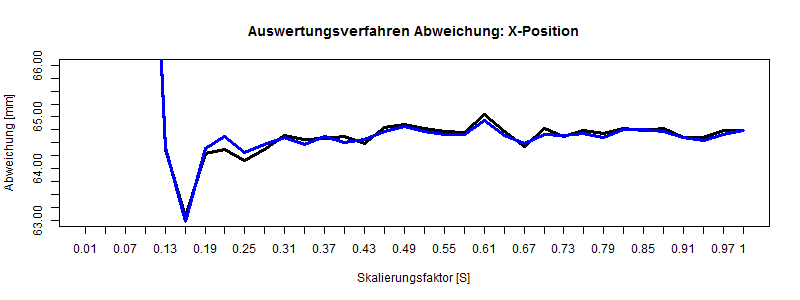
\includegraphics[width=\linewidth]{img_Skalierung/Verfahren_TX}
	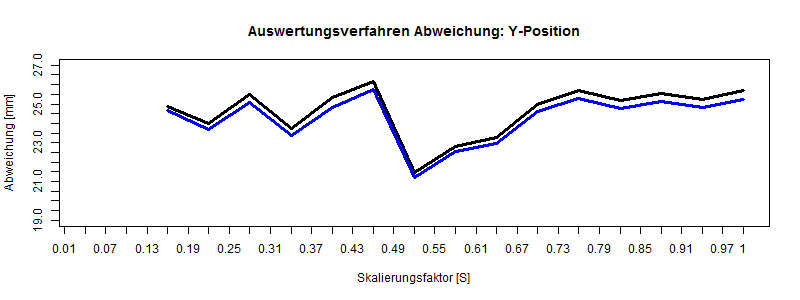
\includegraphics[width=\linewidth]{img_Skalierung/Verfahren_TY}
	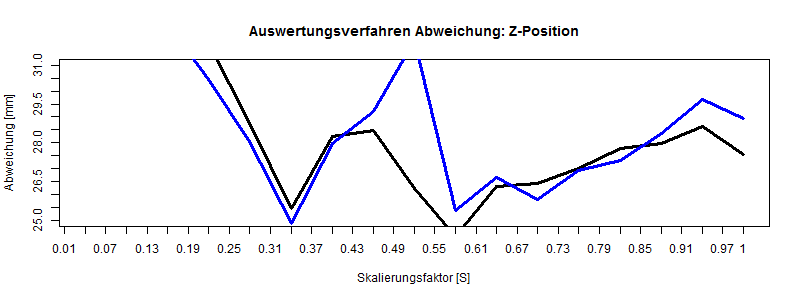
\includegraphics[width=\linewidth]{img_Skalierung/Verfahren_TZ}
	\caption{Median der Abweichung in Millimeter der Positionsbestimmung auf BIWI \cite{database_Face_Ori} die mit Lanczos skaliert wurden.\\
	PoseWorld (schwarz), PoseCamera (rot, verdeckt von PW), CorrectPoseCamera (grün, verdeckt von CPW) und CorrectPoseWorld (blau)\\
	Oben: X-Position, Mitte: Y-Position, Unten: Z-Position}
	\label{img_Verfahren_Pos}
\end{figure}
\subsubsection{Orientierung}
Bei der Rotation zeigen sich nun Unterschiede zwischen den einzelnen Verfahren, da bei PoseWorld und CorrectPoseWorld auch die Position im Kamerabild berücksichtigt wird.\\
Aus \autoref{img_Verfahren_Rot} ist zu entnehmen, dass die zusätzliche Korrektur das Ergebnis weiter verbessert, wenn die Pixelorientierungen mit beachtet werden.
\begin{figure}
	\centering
	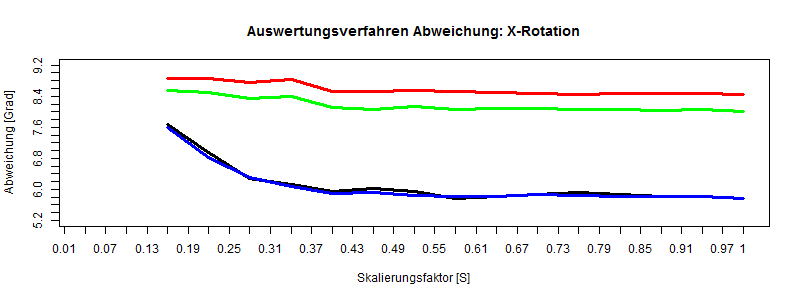
\includegraphics[width=\linewidth]{img_Skalierung/Verfahren_RX}
	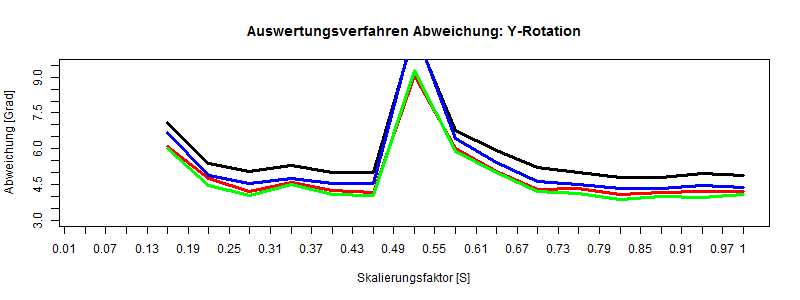
\includegraphics[width=\linewidth]{img_Skalierung/Verfahren_RY}
	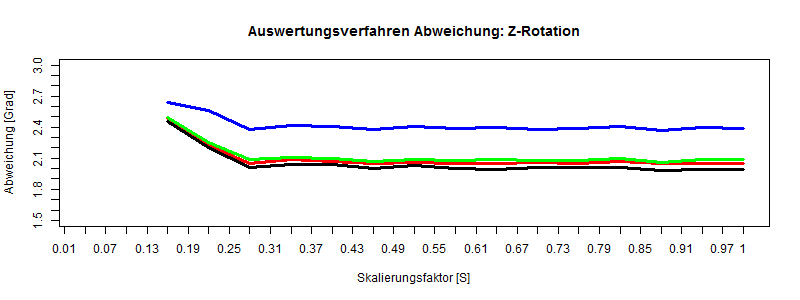
\includegraphics[width=\linewidth]{img_Skalierung/Verfahren_RZ}
	\caption{Dargestellt ist der Median der Abweichung in Grad der Positionsbestimmung auf Bilder die mit Lanczos skaliert wurden.\\
		PoseWorld (schwarz), PoseCamera (rot), CorrectPoseCamera (grün) und CorrectPoseWorld (blau)\\
		Oben: X-Rotation, Mitte: Y-Rotation, Unten: Z-Rotation}
	\label{img_Verfahren_Rot}
\end{figure}
\subsubsection{Ergebnis}
Es zeigt sich, dass PoseWorld, also die einfache Bestimmung der Position mittels Skalierung und Brennweite und zusätzlicher Korrektur der Winkel die besten Ergebnisse liefert im Test.\\
Im Test ist die Überführung von 3D zu 2D Landmarks in manchen Parametern (z.B. Y-Rotation) überlegen, wobei der unterschied minimal ausfällt. Dies kann sich allerdings auch ändern wenn die Kamera Parameter besser abgeschätzt sind, da ohne eine Tiefenaufnahme die korrekte Überführung nur geschätzt werden kann und sich Fehler fortpflanzen können.